\documentclass[tikz,{2cm 1pt 2cm 1pt}]{standalone}
\usepackage{tikz}
\usepackage{amsmath}
\usepackage{bm}

\usetikzlibrary{calc,angles,quotes}

\begin{document}

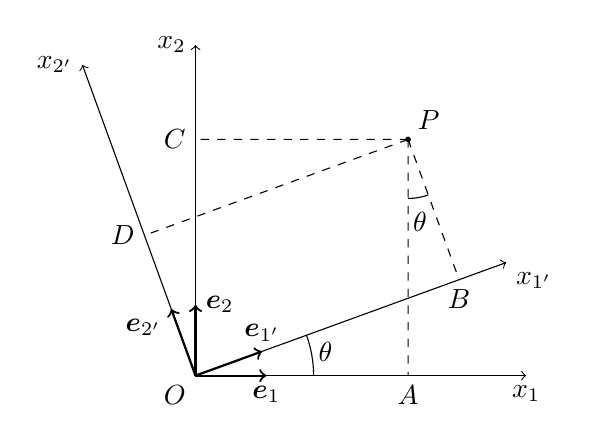
\begin{tikzpicture}[scale=3]

% rotation angle
\def\teta{20}

% axes length
\def\L{1.4}
\def\eL{0.3}

% origin
\coordinate (O) at (0,0);
\node[below left] at (O) {$O$};

% reference axes
\coordinate (X1) at (\L,0);
\coordinate (X2) at (0,\L);

\draw[->,thin] (O) -- (X1) node[below] {$x_1$};
\draw[->,thin] (O) -- (X2) node[left] {$x_2$};

% rotated axes
\coordinate (X1p) at ({\L*cos(\teta)},{\L*sin(\teta)});
\coordinate (X2p) at ({-\L*sin(\teta)},{\L*cos(\teta)});

\draw[->,thin] (O) -- (X1p) node[below right] {$x_{1'}$};
\draw[->,thin] (O) -- (X2p) node[left] {$x_{2'}$};

% reference base vectors
\coordinate (eX1) at (\eL,0);
\coordinate (eX2) at (0,\eL);

\draw[->,thick] (O) -- (eX1) node[below] {$\boldsymbol{e}_1$};
\draw[->,thick] (O) -- (eX2) node[right] {$\boldsymbol{e}_2$};

% rotated base vectors
\coordinate (eX1p) at ({\eL*cos(\teta)},{\eL*sin(\teta)});
\coordinate (eX2p) at ({-\eL*sin(\teta)},{\eL*cos(\teta)});

\draw[->,thick] (O) -- (eX1p) node[above] {$\boldsymbol{e}_{1'}$};
\draw[->,thick] (O) -- (eX2p) node[below left] {$\boldsymbol{e}_{2'}$};

% point P
\coordinate (P) at (0.9,1);
\fill (P) circle (0.012);
\node[above right] at (P) {$P$};

% projections onto reference axes
\coordinate (Px1) at ($(O)!(P)!(X1)$);
\draw[dashed] (P) -- (Px1);
\node[below] at (Px1) {$A$};

\coordinate (Px2) at ($(O)!(P)!(X2)$);
\draw[dashed] (P) -- (Px2);
\node[left] at (Px2) {$C$};


% projections onto rotated axes
\coordinate (Px1p) at ($(O)!(P)!(X1p)$);
\draw[dashed] (P) -- (Px1p);
\node[below] at (Px1p) {$B$};

\coordinate (Px2p) at ($(O)!(P)!(X2p)$);
\draw[dashed] (P) -- (Px2p);
\node[left] at (Px2p) {$D$};

% angle at origin
\draw (0.5,0) arc (0:\teta:0.5);
\node at (0.55,0.1) {$\theta$};

% angle near P
\draw (P) ++(-0,-0.25) arc (-90:-90+\teta:0.25);
\node at ($(P)+(0.05,-0.35)$) {$\theta$};

\end{tikzpicture}

\end{document}
